\documentclass{beamer}

\usetheme{Singapore}

\usepackage{verbatim}
\usepackage{url}
\usepackage{graphicx}

\usepackage{tikz}
\usetikzlibrary{through,calc,intersections}
\usetikzlibrary{arrows.meta,shapes.geometric}
\tikzset{>=stealth}

% Display vertex not affected by tikz scale
\newcommand*{\vertex}[1]
  {\fill[shift only] (#1) circle (1.5pt)}
\newcommand*{\vertexcolor}[2]
  {\fill[shift only,#2] (#1) circle (1.5pt)}

% Very small math, used in drawings
\newcommand*{\sm}[1]{$\scriptstyle #1$}

% In heptdecagon chapter, stack numbers of occurrences, variables
\newcommand*{\occ}[2]{\underset{#2\quad}{r^{#1}}}

\title{Mathematical Surprises}
\author{Moti Ben-Ari\\\url{https://www.weizmann.ac.il/sci-tea/benari}}
\institute{Department of Science Teaching\\
Weizmann Institute of Science}
\date{}


\begin{document}

\frame{\titlepage}

%%%%%%%%%%%%%%%%%%%%%%%%%%%%%%%%%%%%%%%%%%%%%%%%%%%%%%

\begin{frame}
\begin{center}
\vspace*{-5ex}
\includegraphics[height=7cm]{surprises-cover}
\end{center}
\small\url{https://link.springer.com/book/10.1007/978-3-031-13566-8}

\medskip

\small\url{https://github.com/motib/surprises}
\end{frame}

%%%%%%%%%%%%%%%%%%%%%%%%%%%%%%%%%%%%%%%%%%%%%%%%%%%%%%

\begin{frame}
\frametitle{Criteria}

\begin{itemize}
\item Surprising
\item Does not appear in secondary-school / college textbooks
\item Accessible with secondary-school mathematics
\end{itemize}

\end{frame}

%%%%%%%%%%%%%%%%%%%%%%%%%%%%%%%%%%%%%%%%%%%%%%%%%%%%%%


\begin{frame}
\frametitle{Constructions With Straightedge and Compass}

\pause

\begin{description}
\item[Possible] Right triangle, bisect an angle, perpendicular bisector

\bigskip

\item[Impossible] Trisect an angle, square a circle, double a cube, regular septagon

\pause

\bigskip

\item[Tools] Neusis, quadratrix
\end{description}
\end{frame}


\begin{frame}
\frametitle{1. The Collapsing Compass}

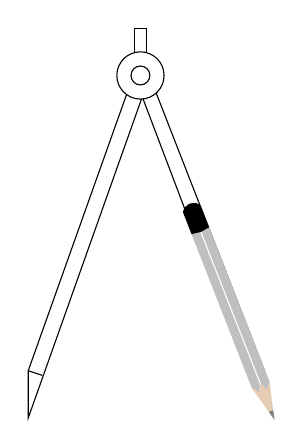
\begin{tikzpicture}
\begin{scope}[rotate=0,transform shape,scale=3]
\draw (2.95,3.7) rectangle (3,3.95);
\draw (2.92,3.68) -- (2.5,2.5) -- (2.5,2.3) -- (2.99,3.68);
\draw (3.5,2.5) -- (3.43,2.48) -- (2.975,3.68);
\draw (3.04,3.68) -- (3.5,2.5);
\draw (2.5,2.5) -- (2.56,2.48);
\draw[fill=white] (2.975,3.75) circle (0.1cm);
\draw (2.975,3.75) circle (0.04cm);
\end{scope}
\begin{scope}[xshift=10.34cm,yshift=7.28cm,rotate=21.4,scale=.6]          
\fill[gray!50] (0,4) -- (0.4,4) -- (0.4,0) --
               (0.3,-0.15) -- (0.2,0) -- (0.1,-0.14) --
               (0,0) -- cycle;
\draw[color=white] (0.2,4) -- (0.2,0);
\fill[black] (0,3.5) -- (0.2,3.47) -- (0.4,3.5) --
             (0.4,4) arc(30:150:0.23cm);
\fill[brown!40] (0,0) -- (0.2,-0.8)
    node[coordinate,pos=0.75](a){} -- 
    (0.4,0)node[coordinate,pos=0.25](b){} -- 
    (0.3,-0.15) -- (0.2,0) -- (0.1,-0.14) -- cycle;
\fill[gray] (a) -- (0.2,-0.8) -- (b) -- cycle;
\end{scope}
\end{tikzpicture}
\hfill
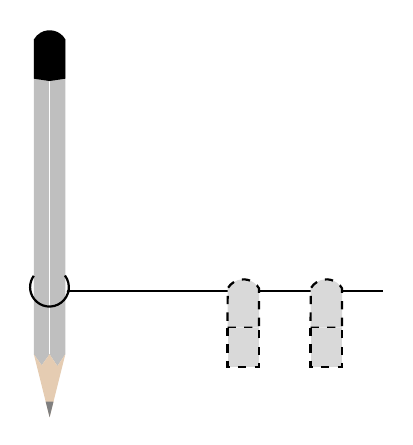
\begin{tikzpicture}[rotate=0,scale=1]          
\fill[gray!50] (0,4) -- (0.4,4) -- (0.4,0) --
               (0.3,-0.15) -- (0.2,0) -- (0.1,-0.14) --
               (0,0) -- cycle;
\draw[color=white] (0.2,4) -- (0.2,0);
\fill[black] (0,3.5) -- (0.2,3.47) -- (0.4,3.5) --
             (0.4,4) arc(30:150:0.23cm);
\fill[brown!40] (0,0) -- (0.2,-0.8)
    node[coordinate,pos=0.75](a){} -- 
    (0.4,0) node[coordinate,pos=0.25](b){} -- 
    (0.3,-0.15) -- (0.2,0) -- (0.1,-0.14) -- cycle;
\fill[gray] (a) -- (0.2,-0.8) -- (b) -- cycle;

\draw[thick] (0.395,1) arc (37:-216:7pt);
\coordinate (knot) at (0.44,.8);
\draw[thick] (knot) -- +(4,0);
\fill (knot) circle (.7pt);

\begin{scope}[xshift=100pt,yshift=-90pt]
\draw[dashed,thick,fill=white!70!gray] (0,3.5) -- (0.4,3.5) -- 
      (0.4,4) arc(30:150:0.23cm) -- cycle;
\draw[dashed,thick,fill=white!70!gray] (0,3.5) -- ++(0,-.5) -- ++(.4,0) -- ++(0,.5);
\end{scope}

\begin{scope}[xshift=70pt,yshift=-90pt]
\draw[dashed,thick,fill=white!70!gray] (0,3.5) -- (0.4,3.5) -- 
      (0.4,4) arc(30:150:0.23cm) -- cycle;
\draw[dashed,thick,fill=white!70!gray] (0,3.5) -- ++(0,-.5) -- ++(.4,0) -- ++(0,.5);
\end{scope}
\end{tikzpicture}

\bigskip

\textit{Theorem (Euclid)} Any construction that can be performed using a fixed compass can be performed using a collapsing compass.

 \end{frame}

%%%%%%%%%%%%%%%%%%%%%%%%%%%%%%%%%%%%%%%%%%%%%%%%%%%%%%

\begin{frame}
\frametitle{2. Trisecting an Angle}

Underwood Dudley. \textit{What To Do When the Trisector Comes}.

\pause

Underwood Dudley. \textit{A Budget of Trisections}.

\medskip

\begin{center}
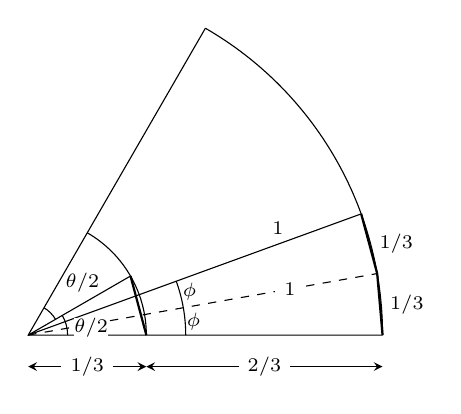
\begin{tikzpicture}[scale=.5]
\coordinate (O) at (0,0)
  node[above right,xshift=10pt,yshift=12pt] {\sm{\theta/2}};
\coordinate (A) at (9cm,0);
\coordinate (B) at (60:9);
\draw (A) arc(0:60:9);
\draw (B) -- (O) -- (A);
\coordinate (D) at (3,0);
\draw[name path=third] (D) arc(0:60:3);
\coordinate (C) at (30:3);
\draw (O) --  (C);
\draw[thick] (D) -- (C);
\coordinate (E) at (10:9);
\draw[thick] (A) -- node[right] {\sm{1/3}} (E);
\coordinate (T) at (20:9);
\draw[thick] (E) -- node[right] {\sm{1/3}} (T);
\draw (O) -- node[above,near end] {\sm{1}} (T);
\draw (	1,0) arc (0:30:1);
\draw (30:.8) arc (30:60:.8);
\draw (4,0) arc (0:20:4);
\node at (4.2,0.35) {\sm{\phi}}; 
\node at (4.1,1.1) {\sm{\phi}}; 
\draw[dashed] (O) --
  node[fill=white,inner sep=0pt,very near start,
       xshift=7pt] {\sm{\theta/2}} 
  node[fill=white,near end] {\sm{1}} (E);
\draw[<->] (3,-.8) -- node[fill=white] {\sm{2/3}} +(6,0);
\draw[<->] (0,-.8) -- node[fill=white] {\sm{1/3}} +(3,0);
\end{tikzpicture}
\end{center}

\medskip

For $\theta=60^\circ$: $2\phi=
2\cos^{-1}\left(1 - \frac{1}{9}(1-\cos 30^\circ)\right)\approx 19.8^\circ\approx 20^\circ$
\end{frame}

%%%%%%%%%%%%%%%%%%%%%%%%%%%%%%%%%%%%%%%%%%%%%%%%%%%%%%

%\begin{frame}
%\frametitle{Trisection Using the Neusis of Archiemedes}
%
%\begin{center}
%\begin{tikzpicture}[scale=2.1]
%\coordinate (origin) at (0,0);
%\draw[name path=circle] (origin) circle [radius=1];
%\draw (origin) -- node[fill=white] {$1$} (120:1) coordinate (a); 
%\draw (-1,0) -- (2.5,0);
%\path[name path=ad] (a) -- (0,0 -| 2,0) coordinate (d);
%\path[name intersections={of=circle and ad,by={c,a1}}];
%\coordinate (e) at (-1,0);
%\draw (origin) -- node[fill=white] {$1$} (c);
%\vertex{origin};
%\begin{scope}[rotate=-19,yshift=-11.25pt]
%\draw (-1,1.05) rectangle +(3.2,.1);
%\draw[thick] (1.89,1.05) -- +(0,.1);
%\draw[thick] (.76,1.05) -- +(0,.1);
%\draw[<->] (.73,1.3) -- node[fill=white] {$1$} (1.89,1.3);
%\end{scope}
%\end{tikzpicture}
%\end{center}
%
%\end{frame}
%%%%%%%%%%%%%%%%%%%%%%%%%%%%%%%%%%%%%%%%%%%%%%%%%%%%%%

\begin{frame}
\frametitle{3. Squaring the Circle}

\medskip

\begin{center}
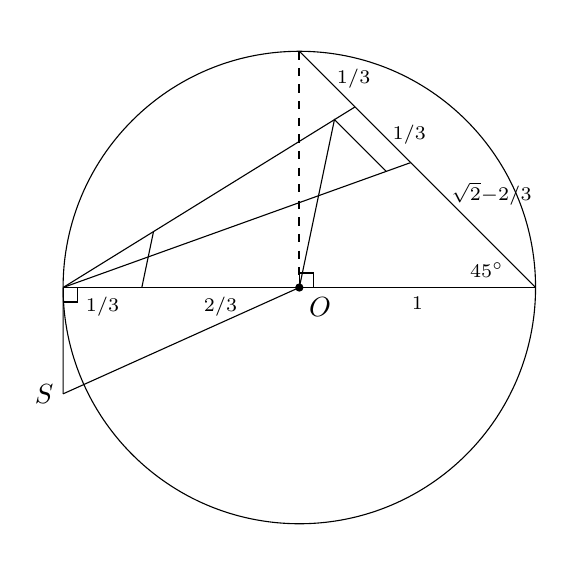
\begin{tikzpicture}[scale=.75]
\clip (-4.6,-4.2) rectangle +(8.8,8.6);
% Scale at 4

% Coordinates of circle
\coordinate (O) at (0,0);
\vertex{O};
\coordinate (A) at (-4,0);
\coordinate (B) at (4,0);
\coordinate (C) at (0,4);

% Draw circle and diameter
\node [draw,circle through=(A),name path=circle] at (O) {};
\draw (A) -- (B);
\draw [thick,dashed] (C) -- (O);
\draw (O) rectangle +(7pt,7pt);
\draw[rotate=-90] (A) rectangle +(7pt,7pt);

\coordinate (T) at (-2.667,0);
\path (A) -- node[below] {\sm{1/3}} (T);
\path (T) -- node[below] {\sm{2/3}} (O);
\path (O) -- node[below] {\sm{1}} (B);

\draw (C) -- node[right] {\sm{1/3}} +(-45:1.333) coordinate (M);
\draw (M) -- node[right] {\sm{1/3}} +(-45:1.333) coordinate (N);
\draw (N) -- node[near start,right] {\sm{\sqrt{2}-2/3}}(B);

\draw[name path=AM] (A) -- (M);
\draw[name path=AN] (A) -- (N);

\node [circle through=(M),name path=AMcircle] at (A) {};

\path[name intersections={of=AMcircle and AN,by=P}];

\path[name path=PQ] (P) -- +(135:2);
\path[name intersections={of=PQ and AM,by=Q}];
\draw (P) -- (Q) -- (O);

\path[name path=QT] (T) -- ($(Q)+(-2.667,0)$) -- (Q);
\path[name intersections={of=QT and AM,by=R}];
\draw (T) -- (R);

\node [circle through=(R),name path=ARcircle] at (A) {};
\path[name path=AS] (A) -- ($(A)+(0,-2.5)$);
\path[name intersections={of=ARcircle and AS,by=S}];
\draw (A) -- (S);

\draw (S) -- (O);

\node[below right] at (O) {$O$};
\node[above left,xshift=-8pt] at (B) {\sm{45^\circ}};
\node[left] at (S) {$S$};
\end{tikzpicture}

Obviously: $\quad 3\sqrt{\overline{SO}}=\left(9^2+\displaystyle\frac{19^2}{22}\right)^{1/4}\approx \pi$
\end{center}

\end{frame}

%%%%%%%%%%%%%%%%%%%%%%%%%%%%%%%%%%%%%%%%%%%%%%%%%%%%%%

%\begin{frame}
%\frametitle{Euler's Formula}
%
%\textit{Theorem} Let $G$ be a connected \textit{planar} graph with $V$ vertices, $E$ edges and $F$ faces. Then $V-E+F=2$.
%
%\medskip
%
%\begin{center}
%\begin{tikzpicture}[scale=.6]
%\coordinate (O) at (0,0);
%\foreach \x/\name/\n/\po in {0/a/A/right,.6/b/B/above,1.6/c/C/left,2.4/d/D/below left,3.9/e/E/below right} {
%  \coordinate (\name) at ($(O)+(\x*72+18:3cm)$);
%\draw (O) -- (\name);
%}
%\vertex{O};
%\vertex{a};
%\vertex{b};
%\vertex{c};
%\vertex{d};
%\vertex{e};
%\draw (a) -- (b) -- (c) -- (d) --(e) -- cycle;
%\end{tikzpicture}
%\end{center}
%
%\[
%6-10+6=2
%\]
%
%\medskip
%
%\pause
%
%\textit{Theorem}
%There is a vertex with less than six neighbors.
%
%\end{frame}

\begin{frame}
\frametitle{4. The Five-Color Theorem}

\textit{Theorem}
There is a vertex with less than six neighbors.

\textit{Proof} Use Euler's formula for planar graphs: $V-E+F=2$.

\medskip

\begin{center}
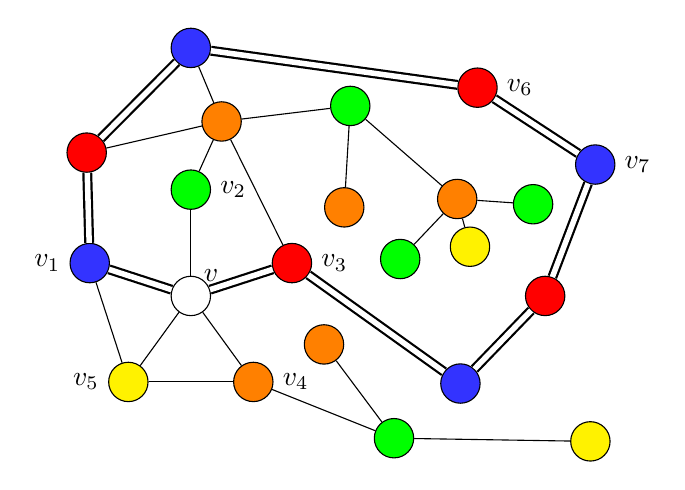
\begin{tikzpicture}[scale=.45,minimum size=5mm,inner sep=0pt]
\foreach \name/\color/\theta in
    {A/red/18,B/green/90,C/blue!80/162,D/yellow/234,E/orange/306}
  \node[circle,draw,fill=\color] (\name) at (\theta:3) {};
\node[circle,draw] (O) at (0,0) {};
\node[above right] at (O) {$v$};

\node[right,xshift=8pt] at (A) {$v_3$};
\node[right,xshift=8pt] at (B) {$v_2$};
\node[left,,xshift=-8pt] at (C) {$v_1$};
\node[left,,xshift=-8pt] at (D) {$v_5$};
\node[right,xshift=8pt] at (E) {$v_4$};

\foreach \name in {A,B,C,D,E}
  \draw (O) -- (\name);
  
\node[circle,draw,fill=red]  (X1) at (126:5) {};
\node[circle,draw,fill=blue!80] (X2) at (90:7)  {};
\node[circle,draw,fill=red]  (X3) at (36:10) {};
\node[right,xshift=8pt] at (X3) {$v_6$};
\node[circle,draw,fill=blue!80] (X4) at (18:12) {};
\node[right,xshift=8pt] at (X4) {$v_7$};
\node[circle,draw,fill=red]  (X5) at (0:10) {};
\node[circle,draw,fill=blue!80] (X6) at (-18:8) {};
\draw[thick,double distance=2pt] (C)  -- (X1);
\draw[thick,double distance=2pt] (X1) -- (X2);
\draw[thick,double distance=2pt] (X2) -- (X3);
\draw[thick,double distance=2pt] (X3) -- (X4);
\draw[thick,double distance=2pt] (X4) -- (X5);
\draw[thick,double distance=2pt] (X5) -- (X6);
\draw[thick,double distance=2pt] (X6) -- (A);
\draw[thick,double distance=2pt] (A) -- (O) -- (C);

\node[circle,draw,fill=orange]  (Y1)  at (80:5) {};
\node[circle,draw,fill=green]   (Y2)  at (50:7)  {};
\node[circle,draw,fill=orange]  (Y3A) at (20:8) {};
\node[circle,draw,fill=orange]  (Y3B) at (30:5) {};
\node[circle,draw,fill=green]   (Y4A) at (10:6) {};
\node[circle,draw,fill=yellow]  (Y4B) at (10:8) {};
\node[circle,draw,fill=green]   (Y4C) at (15:10) {};
\node[circle,draw,fill=green]   (Y5)  at (-35:7) {};
\node[circle,draw,fill=yellow]  (Y6A) at (-20:12) {};
\node[circle,draw,fill=orange]  (Y6B) at (-20:4) {};
\draw (B)  -- (Y1);
\draw (Y1) -- (Y2);
\draw (Y2) -- (Y3A);
\draw (Y2) -- (Y3B);
\draw (Y3A) -- (Y4A);
\draw (Y3A) -- (Y4B);
\draw (Y3A) -- (Y4C);
\draw (E)  -- (Y5);
\draw (Y5) -- (Y6A);
\draw (Y5) -- (Y6B);
\draw (A) -- (Y1);
\draw (X2) -- (Y1);
\draw (X1) -- (Y1);
\draw (D) -- (E);
\draw (D) -- (C);
\end{tikzpicture}
\end{center}

\end{frame}

%%%%%%%%%%%%%%%%%%%%%%%%%%%%%%%%%%%%%%%%%%%%%%%%%%%%%%

\begin{frame}
\frametitle{5. How to Guard a Museum}

\begin{center}
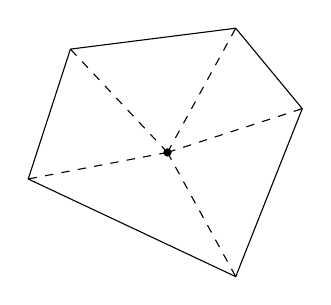
\begin{tikzpicture}[scale=.6]
\coordinate (O) at (0,0);
\vertex{O};
\foreach \x/\name/\n/\po in {0/a/A/right,.6/b/B/above,1.6/c/C/left,2.4/d/D/below left,3.9/e/E/below right} {
  \coordinate (\name) at ($(O)+(\x*72+18:3cm)$);
\draw[dashed] (O) -- (\name);
}
\draw (a) -- (b) -- (c) -- (d) --(e) -- cycle;
\end{tikzpicture}

\pause

\bigskip

$n/3$ guards are necessary

\bigskip

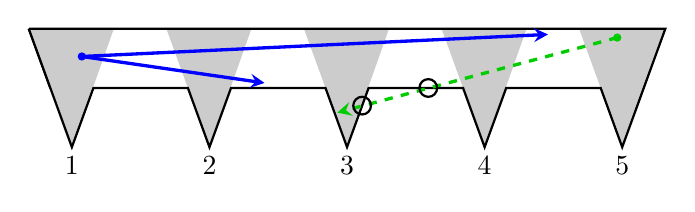
\begin{tikzpicture}[scale=.8]
\coordinate (O) at (0,0);
\draw [thick] (O) -- (++110:1cm) coordinate (P);
\path (O) --
  ++(-70:1cm) coordinate(A) node[below] {$1$} -- 
  ++(+70:1cm) coordinate(A1) -- ++(0:1.5cm) coordinate(A2) --
  ++(-70:1cm) coordinate(B) node[below] {$2$} -- 
  ++(+70:1cm) coordinate(B1) -- ++(0:1.5cm) coordinate(B2) --
  ++(-70:1cm) coordinate(C) node[below] {$3$}-- 
  ++(+70:1cm) coordinate(C1) -- ++(0:1.5cm) coordinate(C2) --
  ++(-70:1cm) coordinate(D) node[below] {$4$} -- 
  ++(+70:1cm) coordinate(D1) -- ++(0:1.5cm) coordinate(D2) --
  ++(-70:1cm) coordinate(E) node[below] {$5$} --
  ++(+70:2cm) coordinate(E1) -- (P);

\path[fill,black!20!white] (A) -- ++(110:2cm) -- ++(0:1.35cm)-- cycle;
\path[fill,black!20!white] (B) -- ++(110:2cm) -- ++(0:1.35cm)-- cycle;
\path[fill,black!20!white] (C) -- ++(110:2cm) -- ++(0:1.35cm)-- cycle;
\path[fill,black!20!white] (D) -- ++(110:2cm) -- ++(0:1.35cm)-- cycle;
\path[fill,black!20!white] (E) -- ++(110:2cm) -- ++(0:1.35cm)-- cycle;

\draw[thick] (P) -- (O) -- (A) -- (A1) -- (A2) --
   (B) -- (B1) -- (B2) -- (C) -- (C1) -- (C2) --
   (D) -- (D1) -- (D2) -- (E) -- (E1) -- (P);

\coordinate (G1) at (9,.8);
\coordinate (G2) at ($(O)+(.5,.5)$);
\draw[->,very thick,green!80!black,dashed] (G1) -- +(-165:4.6cm);
\draw[->,very thick,blue] (G2) -- ++(7.4,.35);
\draw[->,very thick,blue] (G2) -- ++(2.9,-.42);
\draw[thick] (6,0) circle(4pt);
\draw[thick] (4.95,-.28) circle(4pt);
\vertexcolor{G1}{green!80!black};
\vertexcolor{G2}{blue};
\end{tikzpicture}
\end{center}

\end{frame}

%%%%%%%%%%%%%%%%%%%%%%%%%%%%%%%%%%%%%%%%%%%%%%%%%%%%%%

%\begin{frame}
%\frametitle{Proving that $n/3$ Guards are Sufficient}
%\begin{itemize}
%\item Any polygon can be triangulated.
%\item Any triangulated polygon can be three-colored.
%\item All three vertices of a three-colored triangulated polygon must be colored with different colors.
%\item One guard per triangle can see the entire interior of all triangles.
%\end{itemize}
%\end{frame}

%%%%%%%%%%%%%%%%%%%%%%%%%%%%%%%%%%%%%%%%%%%%%%%%%%%%%%

\begin{frame}
\frametitle{5. How to Guard a Museum}

\textit{Theorem} $n/3$ Guards are Sufficient

\textit{Proof} By induction on three-coloring triangulated polygons.

\bigskip
\bigskip

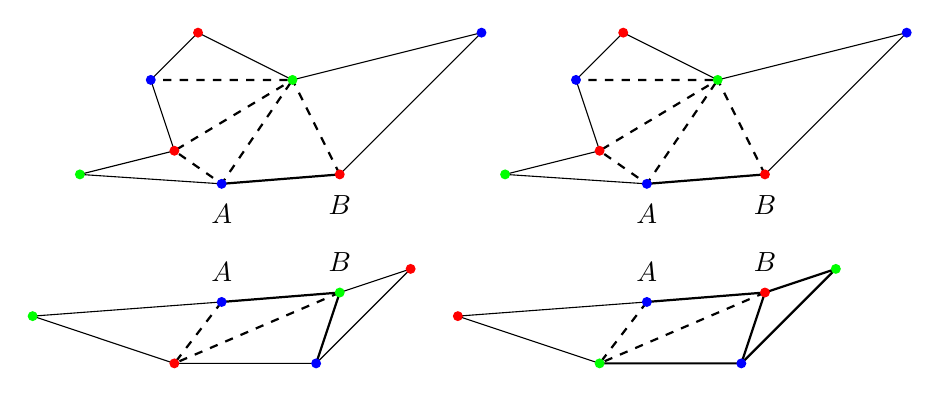
\begin{tikzpicture}[scale=.6]
\path
  (0,0) coordinate (A1) -- 
  ++(3,0) coordinate (B1) --
  ++(2,2) coordinate (C1) --
  ++(-1.5,-.5) coordinate (D1);
\draw
  (D1) --
  ++(3,3) coordinate (E1) -- 
  ++(-4,-1) coordinate (F1) --
  ++(-2,1) coordinate (G1) --
  ++(-1,-1) coordinate (H1) --
  ++(.5,-1.5) coordinate (I1) --
  ++(-2,-.5) coordinate (J1) --
  ++(3,-.2) coordinate (K1);
\path
  (K1) -- 
  ++(-4,-.3) coordinate (L1) --
  (A1);
  
\draw[thick,dashed]
  (D1) -- (F1) -- (I1) -- (K1) -- (F1) -- (H1);
\draw[thick] (D1) -- (K1);

\node[below,yshift=-4pt] at (K1) {$A$};
\node[below,yshift=-4pt] at (D1) {$B$};

\foreach \point/\color in {D1/red,E1/blue,F1/green,G1/red,H1/blue,I1/red,J1/green,K1/blue}
  \fill[color=\color] (\point) circle(3pt);

\begin{scope}[yshift=-2.5cm]

\draw
  (0,0) coordinate (A2) -- 
  ++(3,0) coordinate (B2) --
  ++(2,2) coordinate (C2) --
  ++(-1.5,-.5) coordinate (D2);
\path
  (D2) --
  ++(3,3) coordinate (E2) --
  ++(-4,-1) coordinate (F2) --
  ++(-2,1) coordinate (G2) --
  ++(-1,-1) coordinate (H2) --
  ++(.5,-1.5) coordinate (I2) --
  ++(-2,-.5) coordinate (J2) --
  ++(3,-.2) coordinate (K2);
\draw
  (K2) --
  ++(-4,-.3) coordinate (L2) --
  (A2);
  
\draw[thick,dashed]
  (K2) -- (A2) -- (D2) -- (B2) -- (D2);
\draw[thick] (D2) -- (K2);
\node[above,yshift=4pt] at (K2) {$A$};
\node[above,yshift=4pt] at (D2) {$B$};

\foreach \point/\color in {A2/red,B2/blue,C2/red,D2/green,K2/blue,L2/green}
  \fill[color=\color] (\point) circle(3pt);

\end{scope}

\begin{scope}[xshift=9cm]
\path
  (0,0) coordinate (A1) -- 
  ++(3,0) coordinate (B1) --
  ++(2,2) coordinate (C1) --
  ++(-1.5,-.5) coordinate (D1);
\draw
  (D1) --
  ++(3,3) coordinate (E1) -- 
  ++(-4,-1) coordinate (F1) --
  ++(-2,1) coordinate (G1) --
  ++(-1,-1) coordinate (H1) --
  ++(.5,-1.5) coordinate (I1) --
  ++(-2,-.5) coordinate (J1) --
  ++(3,-.2) coordinate (K1);
\path
  (K1) -- 
  ++(-4,-.3) coordinate (L1) --
  (A1);
  
\node[below,yshift=-4pt] at (K1) {$A$};
\node[below,yshift=-4pt] at (D1) {$B$};

\draw[thick,dashed]
  (D1) -- (F1) -- (I1) -- (K1) -- (F1) -- (H1);
\draw[thick] (D1) -- (K1);

\foreach \point/\color in {D1/red,E1/blue,F1/green,G1/red,H1/blue,I1/red,J1/green,K1/blue}
  \fill[color=\color] (\point) circle(3pt);

\begin{scope}[yshift=-2.5cm]

\draw[thick]
  (0,0) coordinate (A2) -- 
  ++(3,0) coordinate (B2) --
  ++(2,2) coordinate (C2) --
  ++(-1.5,-.5) coordinate (D2);
\path
  (D2) --
  ++(3,3) coordinate (E2) --
  ++(-4,-1) coordinate (F2) --
  ++(-2,1) coordinate (G2) --
  ++(-1,-1) coordinate (H2) --
  ++(.5,-1.5) coordinate (I2) --
  ++(-2,-.5) coordinate (J2) --
  ++(3,-.2) coordinate (K2);
\draw
  (K2) --
  ++(-4,-.3) coordinate (L2) --
  (A2);
  
\draw[thick,dashed]
  (K2) -- (A2) -- (D2) -- (B2) -- (D2);
\draw[thick] (D2) -- (K2);
\node[above,yshift=4pt] at (K2) {$A$};
\node[above,yshift=4pt] at (D2) {$B$};

\foreach \point/\color in {A2/green,B2/blue,C2/green,D2/red,K2/blue,L2/red}
  \fill[color=\color] (\point) circle(3pt);

\end{scope}
\end{scope}
\end{tikzpicture}

\end{frame}

%%%%%%%%%%%%%%%%%%%%%%%%%%%%%%%%%%%%%%%%%%%%%%%%%%%%%%

\begin{frame}
\frametitle{6. Induction}
\begin{itemize}
\item Fibonacci numbers: $f_n < \left(\displaystyle\frac{7}{4}\right)^n$
\item Fermat numbers: For $n\geq 2$, the last digit of $F_n$ is $7$

%\pause

\item McCarthy's $91$-functionL
\begin{eqnarray*}
f(x) &=& \textrm{\sf if}\;\; x > 100 \;\;\textrm{\sf then}\;\; x - 10 \;\;\textrm{\sf else}\;\; f\,(f\,(x+11))\\
g(x) &=& \textrm{\sf if}\;\; x > 100 \;\;\textrm{\sf then}\;\; x - 10 \;\;\textrm{\sf else}\;\; 91
\end{eqnarray*}

%\pause

\item Josephus problem

\medskip

\textit{Definition} $J(n,q)$ is the position of the survivor out of $n$ is every $q$ is eliminated.

\medskip

\textit{Theorem} $J(n,2)=2t+1$.
\end{itemize}
\end{frame}

%%%%%%%%%%%%%%%%%%%%%%%%%%%%%%%%%%%%%%%%%%%%%%%%%%%%%%

\begin{frame}
\frametitle{7. Solving Quadratic Equations}

Al-Khwarizmi's geometric solution of $x^2+bx=c$

\bigskip

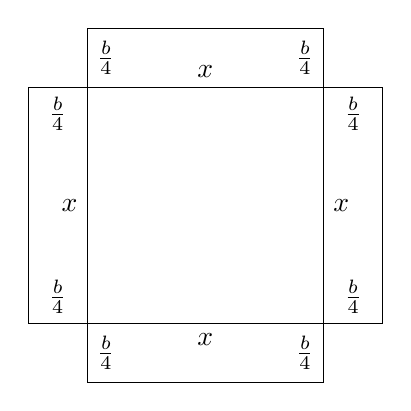
\begin{tikzpicture}[scale=.75]
\coordinate (A) at (0,0);
\coordinate (B) at (4,0);
\coordinate (C) at (4,4);
\coordinate (D) at (0,4);
\draw (A) -- node[below] {$x$} (B) -- node[right] {$x$} (C) -- node[above] {$x$} (D) -- node[left] {$x$} cycle;
\draw (A) -- node[right] {$\frac{b}{4}$} ++(0,-1) -- ++(4,0) -- node[left] {$\frac{b}{4}$} ++(0,1);
\draw (B) -- node[above] {$\frac{b}{4}$} ++(1,0) -- ++(0,4) -- node[below] {$\frac{b}{4}$} ++(-1,0);
\draw (C) -- node[left] {$\frac{b}{4}$} ++(0,1) -- ++(-4,0) -- node[right] {$\frac{b}{4}$} ++(0,-1);
\draw (D) -- node[below] {$\frac{b}{4}$} ++(-1,0) -- ++(0,-4) -- node[above] {$\frac{b}{4}$} ++(1,0);
\end{tikzpicture}
\hspace{2em}
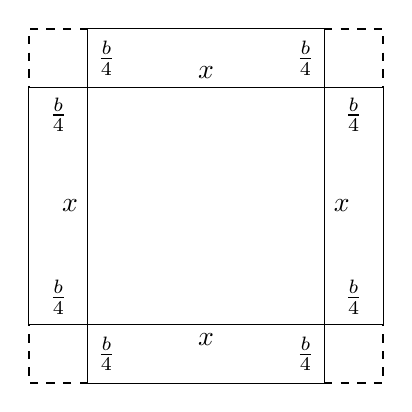
\begin{tikzpicture}[scale=.75]
\coordinate (A) at (0,0);
\coordinate (B) at (4,0);
\coordinate (C) at (4,4);
\coordinate (D) at (0,4);
\draw (A) -- node[below] {$x$} (B) -- node[right] {$x$} (C) -- node[above] {$x$} (D) -- node[left] {$x$} cycle;
\draw (A) -- node[right] {$\frac{b}{4}$} ++(0,-1) -- ++(4,0) -- node[left] {$\frac{b}{4}$} ++(0,1);
\draw (B) -- node[above] {$\frac{b}{4}$} ++(1,0) -- ++(0,4) -- node[below] {$\frac{b}{4}$} ++(-1,0);
\draw (C) -- node[left] {$\frac{b}{4}$} ++(0,1) -- ++(-4,0) -- node[right] {$\frac{b}{4}$} ++(0,-1);
\draw (D) -- node[below] {$\frac{b}{4}$} ++(-1,0) -- ++(0,-4) -- node[above] {$\frac{b}{4}$} ++(1,0);
\draw[thick,dashed] ($(A)+(0,-1)$) -- ++(-1,0) -- ++(0,1);
\draw[thick,dashed] ($(B)+(0,-1)$) -- ++(1,0) -- ++(0,1);
\draw[thick,dashed] ($(C)+(0,1)$) -- ++(1,0) -- ++(0,-1);
\draw[thick,dashed] ($(D)+(0,1)$) -- ++(-1,0) -- ++(0,-1);
\end{tikzpicture}

\bigskip

\begin{center}
$x^2+4(b/4)x$ \hspace{4em} $\quad x^2+4(b/4)x+4(b/4)^2=c+(b^2/4)$
\end{center}
\end{frame}

%%%%%%%%%%%%%%%%%%%%%%%%%%%%%%%%%%%%%%%%%%%%%%%%%%%%%%

\begin{frame}
\frametitle{Cardano's Construction for Cubic Equations}
\begin{center}
\vspace{-3ex}
\[
(a+b)^3=a^3+3a^2b+3ab^2+b^3=(a^3+b^3)+3ab(a+b)
\]

\pause
\bigskip

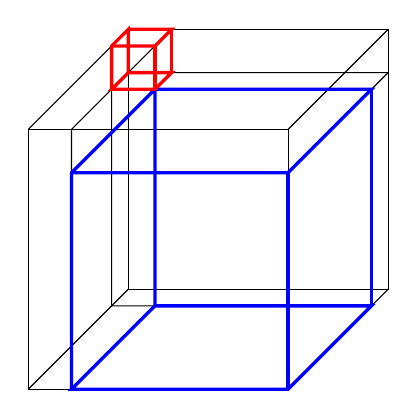
\begin{tikzpicture}[scale=.55]

% Front face
\coordinate (A) at (0,0,0);
%\node[below] at (A) {\sm{0,0,0}};
\coordinate (B) at (6,0,0);
%\node[below right] at (B) {\sm{a+b,0,0}};
\coordinate (C) at (6,6,0);
%\node[above right,xshift=2pt,yshift=-6pt] at (C)
%  {\sm{a+b,a+b,0}};
\coordinate (D) at (0,6,0);
%node[above,xshift=-1pt] at (D) {\sm{0,a+b,0}};

% Front face
\coordinate (FF1) at (1,0,0);
%\node[below] at (FF1) {\sm{b,0,0}};
\coordinate (FF2) at (1,5,0);
%\node[left] at (FF2) {\sm{b,a,0}};
\coordinate (FF3) at (1,6,0);
%\node[below left] at (FF3) {\sm{b,a+b,0}};
\coordinate (FF4) at (6,5,0);
%\node[right] at (FF4) {\sm{a+b,a,0}};

% Back face
\coordinate (A1) at (0,0,-6);
%\node[left,xshift=-1pt] at (A1) {\sm{0,0,a+b}};
\coordinate (B1) at (6,0,-6);
%\node[above,xshift=-3pt] at (B1) {\sm{a+\:b,0,a+b}};
\coordinate (C1) at (6,6,-6);
%\node[above,xshift=-5pt] at (C1) {\sm{a+b,a+b,a+b}};
\coordinate (D1) at (0,6,-6);
%\node[left] at (D1) {\sm{0,a+b,a+b}};

% Back face
\coordinate (BF1) at (0,5,-6);
%\node[above left,xshift=4pt,yshift=-3pt] at (BF1) 
%  {\sm{0,a,a+b}};
\coordinate (BF2) at (1,5,-6);
%\node[below right,xshift=-2pt,yshift=2pt] at (BF2)
%  {\sm{b,a,a+b}};
\coordinate (BF3) at (1,6,-6);
%\node[above] at (BF3) {\sm{b,a+b,a+b}};
\coordinate (BF4) at (6,5,-6);
%\node[above,xshift=-2pt] at (BF4) {\sm{a+b,a,a+b}};

% Right face
\coordinate (RF1) at (6,5,-5);
%\node[right,xshift=1pt] at (RF1) {\sm{a+b,a,a}};
\coordinate (RF2) at (6,0,-5);
%\node[right] at (RF2) {\sm{a+b,0,a}};

% Bottom face
\coordinate (BT1) at (1,0,-5);
%\node[below right] at (BT1) {\sm{b,0,a}};

% Left face
\coordinate (LF1) at (0,0,-5);
%\node[left] at (LF1) {\sm{0,0,a}};
\coordinate (LF2) at (0,5,-5);
%\node[left] at (LF2) {\sm{0,a,a}};
\coordinate (LF3) at (0,6,-5);
%\node[left] at (LF3) {\sm{0,a+b,a}};

% Top face
\coordinate (TF1) at (1,6,-5);
%\node[right,xshift=-2pt,yshift=-2pt] at (TF1) {\sm{b,a+b,a}};

% Internal point
\coordinate (I) at (1,5,-5);
%\node[below right] at (I) {\sm{b,a,a}};


\draw (A) -- (B) -- (C) -- (D) -- cycle;
\draw (A1) -- (B1) -- (C1) -- (D1) -- cycle;
\draw (A) -- (A1);
\draw (B) -- (B1);
\draw (C) -- (C1);
\draw (D) -- (D1);

\draw (FF1) -- (FF2) -- (FF3) -- (BF3);
\draw (BF2) -- (FF2) -- (FF4) -- (BF4);
\draw (FF1) -- (BT1) -- (TF1);
\draw (BF3) -- (BF2);
\draw (TF1) -- (LF3);
\draw (LF3) -- (LF1) -- (RF2) -- (RF1) -- (LF2) -- 
      (BF1) -- (BF4);

\draw[very thick,blue] (FF1) -- (B) -- (RF2) -- (BT1) -- cycle; 
\draw[very thick,blue] (FF1) -- (FF2) -- (I) -- (BT1);
\draw[very thick,blue] (I) -- (RF1) -- (FF4) -- (FF2);
\draw[very thick,blue] (FF4) -- (B);
\draw[very thick,blue] (RF1) -- (RF2);

\draw[very thick,red] (I) -- (LF2) -- (BF1) -- (BF2) -- cycle;
\draw[very thick,red] (LF2) -- (LF3) -- (D1) -- (BF1);
\draw[very thick,red] (D1) -- (BF3) -- (TF1) -- (LF3);
\draw[very thick,red] (TF1) -- (I);
\draw[very thick,red] (BF3) -- (BF2);

\end{tikzpicture}
\hfill
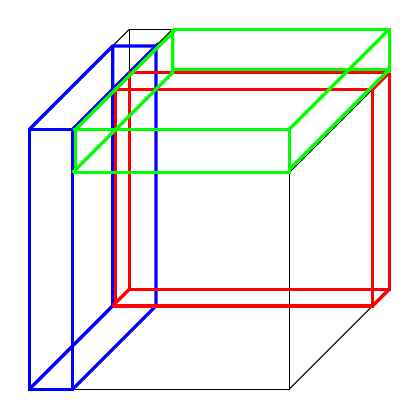
\begin{tikzpicture}[scale=.55]

% Front face
\coordinate (A) at (0,0,0);
%\node[below] at (A) {\sm{0,0,0}};
\coordinate (B) at (6,0,0);
%\node[below right] at (B) {\sm{a+b,0,0}};
\coordinate (C) at (6,6,0);
%\node[above right,xshift=2pt,yshift=-6pt] at (C)
%  {\sm{a+b,a+b,0}};
\coordinate (D) at (0,6,0);
%\node[above,xshift=-1pt] at (D) {\sm{0,a+b,0}};

% Front face
\coordinate (FF1) at (1,0,0);
%\node[below] at (FF1) {\sm{b,0,0}};
\coordinate (FF2) at (1,5,0);
%\node[left] at (FF2) {\sm{b,a,0}};
\coordinate (FF3) at (1,6,0);
%\node[below left] at (FF3) {\sm{b,a+b,0}};
\coordinate (FF4) at (6,5,0);
%\node[right] at (FF4) {\sm{a+b,a,0}};

% Back face
\coordinate (A1) at (0,0,-6);
%\node[left,xshift=-1pt] at (A1) {\sm{0,0,a+b}};
\coordinate (B1) at (6,0,-6);
%\node[above,xshift=-3pt] at (B1) {\sm{a+\:b,0,a+b}};
\coordinate (C1) at (6,6,-6);
%\node[above,xshift=-5pt] at (C1) {\sm{a+b,a+b,a+b}};
\coordinate (D1) at (0,6,-6);
%\node[left] at (D1) {\sm{0,a+b,a+b}};

% Back face
\coordinate (BF1) at (0,5,-6);
%\node[above left,xshift=4pt,yshift=-3pt] at (BF1) 
%  {\sm{0,a,a+b}};
\coordinate (BF2) at (1,5,-6);
%\node[below right,xshift=-2pt,yshift=2pt] at (BF2)
%  {\sm{b,a,a+b}};
\coordinate (BF3) at (1,6,-6);
%\node[above] at (BF3) {\sm{b,a+b,a+b}};
\coordinate (BF4) at (6,5,-6);
%\node[above,xshift=-2pt] at (BF4) {\sm{a+b,a,a+b}};

% Right face
\coordinate (RF1) at (6,5,-5);
%\node[right,xshift=1pt] at (RF1) {\sm{a+b,a,a}};
\coordinate (RF2) at (6,0,-5);
%\node[right] at (RF2) {\sm{a+b,0,a}};

% Bottom face
\coordinate (BT1) at (1,0,-5);
%\node[below right] at (BT1) {\sm{b,0,a}};

% Left face
\coordinate (LF1) at (0,0,-5);
%\node[left] at (LF1) {\sm{0,0,a}};
\coordinate (LF2) at (0,5,-5);
%\node[left] at (LF2) {\sm{0,a,a}};
\coordinate (LF3) at (0,6,-5);
%\node[left] at (LF3) {\sm{0,a+b,a}};

% Top face
\coordinate (TF1) at (1,6,-5);
%\node[right,xshift=-2pt,yshift=-2pt] at (TF1) {\sm{b,a+b,a}};

% Internal point
\coordinate (I) at (1,5,-5);
%\node[below right] at (I) {\sm{b,a,a}};


\draw (A) -- (B) -- (C) -- (D) -- cycle;
\draw (A1) -- (B1) -- (C1) -- (D1) -- cycle;
\draw (A) -- (A1);
\draw (B) -- (B1);
\draw (C) -- (C1);
\draw (D) -- (D1);

\draw (FF1) -- (FF2) -- (FF3) -- (BF3);
\draw (BF2) -- (FF2) -- (FF4) -- (BF4);
\draw (FF1) -- (BT1) -- (TF1);
\draw (BF3) -- (BF2);
\draw (TF1) -- (LF3);
\draw (LF3) -- (LF1) -- (RF2) -- (RF1) -- (LF2) -- 
      (BF1) -- (BF4);

\draw[very thick,blue] (A) -- (FF1) -- (FF3) -- (D) -- cycle;
\draw[very thick,blue] (FF1) -- (BT1) -- (TF1) -- (FF3);
\draw[very thick,blue] (TF1) -- (LF3) -- (D);
\draw[very thick,blue] (LF3) -- (LF1) -- (A);
\draw[very thick,blue] (LF1) -- (BT1);

\draw[very thick,red] (LF1) -- (RF2) -- (RF1) -- (LF2);
\draw[very thick,red] ($(LF2) + (2pt,0)$) -- ($(LF1) + (2pt,0)$);
\draw[very thick,red] (A1) -- (B1) -- (BF4) -- (BF1) -- cycle;
\draw[very thick,red] ($(LF2) + (2pt,0)$) -- ($(BF1) + (2pt,0)$);
\draw[very thick,red] (BF4) -- (RF1);
\draw[very thick,red] (B1) -- (RF2);
\draw[very thick,red] (A1) -- (LF1);

\draw[very thick,green] (FF2) -- (FF4) -- (C) -- (FF3);
\draw[very thick,green] 
  ($(FF2) + (2pt,0)$) -- ($(FF3) + (2pt,0)$);
\draw[very thick,green] 
  ($(FF4) + (0,2pt)$) -- ($(BF4) + (0,2pt)$);
\draw[very thick,green] (BF4) -- (C1) -- (BF3);
\draw[very thick,green] 
  ($(BF3) + (2pt,0)$) -- ($(FF3) + (2pt,0)$);
\draw[very thick,green] (C1) -- (C);
\draw[very thick,green] (BF3) -- (BF2) -- (FF2);
\draw[very thick,green] 
  ($(BF2) + (0,2pt)$) -- ($(BF4) + (0,2pt)$);
\end{tikzpicture}
\end{center}

\end{frame}

%%%%%%%%%%%%%%%%%%%%%%%%%%%%%%%%%%%%%%%%%%%%%%%%%%%%%%

\begin{frame}
\frametitle{8. Ramsey Theory}

$K_5$ \textit{can} be two-colored without a monochromatic $K_3$ (triangle)

\medskip

$K_6$ \textit{cannot} be two-colored without a monochromatic $K_3$ (triangle)

\bigskip

\begin{center}
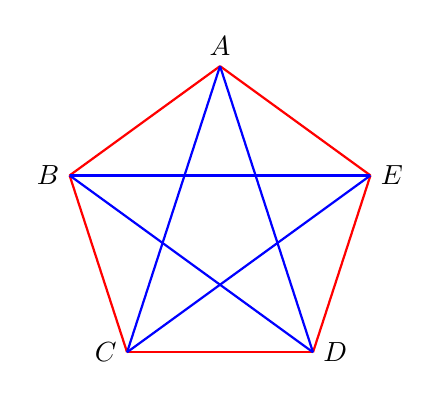
\begin{tikzpicture}
\node (pentagon) [minimum size=4cm,regular polygon,regular polygon sides=5] at (0,0) {};
\draw[red,thick]  (pentagon.corner 1) node[black,above] {$A$} -- (pentagon.corner 2);
\draw[red,thick]  (pentagon.corner 2) node[black,left] {$B$} -- (pentagon.corner 3);
\draw[red,thick]  (pentagon.corner 3) node[black,left] {$C$} -- (pentagon.corner 4);
\draw[red,thick]  (pentagon.corner 4) node[black,right] {$D$} -- (pentagon.corner 5);
\draw[red,thick]  (pentagon.corner 5) node[black,right] {$E$} -- (pentagon.corner 1);
\draw[blue,thick] (pentagon.corner 1) -- (pentagon.corner 3);
\draw[blue,thick] (pentagon.corner 1) -- (pentagon.corner 4);
\draw[blue,thick] (pentagon.corner 2) -- (pentagon.corner 4);
\draw[blue,thick] (pentagon.corner 2) -- (pentagon.corner 5);
\draw[blue,thick] (pentagon.corner 3) -- (pentagon.corner 5);
\end{tikzpicture}
\hspace{1em}
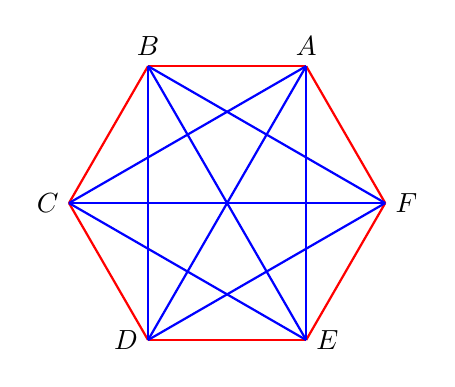
\begin{tikzpicture}
\node (hexagon) [minimum size=4cm,regular polygon,regular polygon sides=6] at (0,0) {};
\draw[red,thick]  (hexagon.corner 1) node[black,above] {$A$} -- (hexagon.corner 2);
\draw[red,thick]  (hexagon.corner 2) node[black,above] {$B$} -- (hexagon.corner 3);
\draw[red,thick]  (hexagon.corner 3) node[black,left] {$C$} -- (hexagon.corner 4);
\draw[red,thick]  (hexagon.corner 4) node[black,left] {$D$} -- (hexagon.corner 5);
\draw[red,thick]  (hexagon.corner 5) node[black,right] {$E$} -- (hexagon.corner 6);
\draw[red,thick]  (hexagon.corner 6) node[black,right] {$F$} -- (hexagon.corner 1);
\draw[thick,blue] (hexagon.corner 1) -- (hexagon.corner 3);
\draw[thick,blue] (hexagon.corner 1) -- (hexagon.corner 4);
\draw[thick,blue] (hexagon.corner 1) -- (hexagon.corner 5);
\draw[thick,blue] (hexagon.corner 2) -- (hexagon.corner 4);
\draw[thick,blue] (hexagon.corner 2) -- (hexagon.corner 5);
\draw[thick,blue] (hexagon.corner 2) -- (hexagon.corner 6);
\draw[thick,blue] (hexagon.corner 3) -- (hexagon.corner 5);
\draw[thick,blue] (hexagon.corner 3) -- (hexagon.corner 6);
\draw[thick,blue] (hexagon.corner 4) -- (hexagon.corner 6);
\end{tikzpicture}
\end{center}

\end{frame}

%%%%%%%%%%%%%%%%%%%%%%%%%%%%%%%%%%%%%%%%%%%%%%%%%%%%%%


\begin{frame}
\frametitle{Ramsey's Theorem}
\textit{Definition}
$R(k)$, the \emph{Ramsey number} for $k$, is the smallest number $n$ such that in \emph{any} coloring of $K_{n}$, the complete graph on $n$ vertices, with two colors there is a monochromatic complete subgraph $K_k$.

\bigskip

\textit{Theorem} For all $k$ the Ramsey number $R(k)$ exists.

\[
\begin{array}{r|r}
\hline
k & R(k)\\\hline
3 & 6\\
4 & 18\\
5 & 43\text{--}48\\
6 & 102\text{--}165\\
7 & 205\text{--}540\\
8 & 282\text{--}1870
\end{array}
\]

\end{frame}

%%%%%%%%%%%%%%%%%%%%%%%%%%%%%%%%%%%%%%%%%%%%%%%%%%%%%%

%\begin{frame}
%\frametitle{Ramsey Theory}
%\begin{itemize}
%\item Ramsey's theorem.
%\item Van der Waerden's problem.
%\item Schur triples.
%\item Pythagorean triples.
%\end{itemize}
%\end{frame}

%%%%%%%%%%%%%%%%%%%%%%%%%%%%%%%%%%%%%%%%%%%%%%%%%%%%%%

\begin{frame}
\frametitle{9. Langford's Problem}
\begin{center}

\begin{tikzpicture}[scale=.9]
\draw[rounded corners,fill=green] (0,0)  
  rectangle +(1.6cm,.8cm);
\draw[rounded corners,fill=red]   (2.2,0)
  rectangle +(1.6cm,.8cm);
\draw[rounded corners,fill=blue]  (4.4,0)
  rectangle +(1.6cm,.8cm);
\draw[rounded corners,fill=red]   (6.6,0)
  rectangle +(1.6cm,.8cm);
\draw[rounded corners,fill=green] (8.8,0)
  rectangle +(1.6cm,.8cm);
\draw[rounded corners,fill=blue]  (11,0)
  rectangle +(1.6cm,.8cm);
\end{tikzpicture}
\end{center}

\pause

\bigskip

\textit{Definition (Langford's Problem $L(n)$)} Given the multiset of positive integers: $\{1,1,2,2,3,3,\ldots,n,n\}$, can they be arranged in a sequence such that for $1\leq i \leq n$ there are $i$ numbers between the two occurrences of $i$\:?

\bigskip

\textit{Theorem} $L(n)$ has a solution if and only if $n=4k$ or $n=4k+3$.

\end{frame}

%%%%%%%%%%%%%%%%%%%%%%%%%%%%%%%%%%%%%%%%%%%%%%%%%%%%%%

\begin{frame}
\frametitle{10, 11, 12. Origami}
\begin{itemize}
\item The seven axioms of origami
\item Lill's method and Beloch fold (solve cubic equations)
\item Constructions: trisect an angle, double a cube, nonagon
\end{itemize}
\end{frame}

%%%%%%%%%%%%%%%%%%%%%%%%%%%%%%%%%%%%%%%%%%%%%%%%%%%%%%

\begin{frame}
\frametitle{13. Mohr-Mascheroni Theorem}

\textit{Question} Is a straightedge needed?

\medskip

\textit{Theorem} Any construction with straightedge and compass can be performed with only a compass.

\pause

\bigskip

\begin{center}
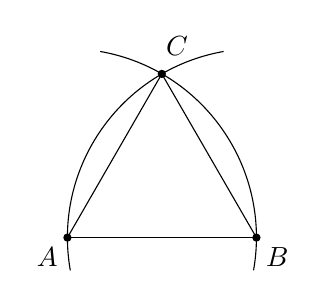
\begin{tikzpicture}[scale=0.6]
\coordinate (A) at (0,0);
\coordinate (B) at (4,0);
\vertex{A};
\vertex{B};
\draw (A) node[below left] {$A$} -- (B) node[below right] {$B$};
\draw[name path=larc] (A) ++(-10:4cm) arc (-10:80:4cm);
\draw[name path=rarc] (B) ++(-170:4cm) arc (-170:-260:4cm);
\path [name intersections={of=larc and rarc,by={t}}];
\node[above right,xshift=-2pt,yshift=3pt] at (t) {$C$};
\vertex{t};
\draw (A) -- (t);
\draw (B) -- (t);
\end{tikzpicture}
\hspace{3em}
\begin{tikzpicture}[scale=0.6]
\coordinate (A) at (0,0);
\coordinate (B) at (4,0);
\vertex{A};
\vertex{B};
\path (A) node[below left] {$A$} -- (B) node[below right] {$B$};
\draw[name path=larc] (A) ++(-10:4cm) arc (-10:80:4cm);
\draw[name path=rarc] (B) ++(-170:4cm) arc (-170:-260:4cm);
\path [name intersections={of=larc and rarc,by={t}}];
\node[above right,xshift=-2pt,yshift=3pt] at (t) {$C$};
\vertex{t};
\end{tikzpicture}
\end{center}

\end{frame}

%%%%%%%%%%%%%%%%%%%%%%%%%%%%%%%%%%%%%%%%%%%%%%%%%%%%%%

\begin{frame}
\frametitle{14. Poncelet-Steiner Theorem}

\textit{Question} Is a compass needed?

\medskip

\textit{Answer} Yes, because the equations of lines are linear.

\bigskip

%\begin{center}
%\begin{tikzpicture}[scale=.4]
%\draw[step=10mm,white!50!black,very thin] (-4,-4) grid (4,4);
%\draw[thick] (-4,0) -- (4,0);
%\draw[thick] (0,-4) -- (0,4);
%\coordinate (O) at (0,0);
%\draw[name path=eq1] (-4,-4) -- (4,4);
%\draw[name path=eq2] (-.5,-4) -- (1.5,4);
%\path[name intersections={of=eq1 and eq2,by={P}}];
%\begin{scope}[xshift=10cm]
%\coordinate (O) at (0,0);
%\draw[step=10mm,white!50!black,very thin] (-4,-4) grid (4,4);
%\draw[thick] (-4,0) -- (4,0);
%\draw[thick] (0,-4) -- (0,4);
%\coordinate (A) at (2,0);
%\node[draw,circle through=(A),name path=circle] at (0,0) {};
%\draw[name path=eq1] (-4,-4) -- (4,4);
%\path[name intersections={of=eq1 and circle,by={P,Q}}];
%\end{scope}
%\begin{scope}[xshift=20cm]
%\coordinate (O) at (0,0);
%\draw[step=10mm,white!50!black,very thin] (-4,-4) grid (4,4);
%\draw[thick] (-4,0) -- (4,0);
%\draw[thick] (0,-4) -- (0,4);
%\coordinate (A) at (3,0);
%\node[draw,circle through=(A),name path=circle1] at (1,0) {};
%\coordinate (B) at (-3,0);
%\node[draw,circle through=(B),name path=circle2] at (-1,0) {};
%\path[name intersections={of=circle1 and circle2,by={P,Q}}];
%\end{scope}
%\end{tikzpicture}
%\end{center}
%
%\pause

\textit{Theorem} Any construction with straightedge and compass can be performed with only a straightedge provided that there is one circle somewhere in the plane.

%\bigskip
%
%\begin{center}
%\begin{tikzpicture}[scale=.75]
%\coordinate (O) at (0,0);
%\node[above right] at (O) {$O$};
%\draw[thick,dashed,name path=circle] (0,0) circle[radius=2cm];
%\draw (0,0) -- node[left] {$r$} ++(-60:2cm);
%\draw[name path=line] (-3,-.5) -- ++(20:6cm);
%\path [name intersections={of=circle and line,by={X,Y}}];
%\node[above right,xshift=-2pt,yshift=4pt] at (X) {$X$};
%\node[above left] at (Y) {$Y$};
%\vertex{O};
%%\vertex{X};
%%\vertex{Y};
%\end{tikzpicture}
%\hspace{2em}
%\begin{tikzpicture}[scale=.75]
%\coordinate (O1) at (0,0);
%\coordinate (O2) at (3,0);
%\node[above right] at (O1) {$O_1$};
%\node[above right] at (O2) {$O_2$};
%\draw[thick,dashed,name path=circle1] (0,0) circle[radius=2cm];
%\draw[thick,dashed,name path=circle2] (3,0) circle[radius=1.7cm];
%\draw (0,0) -- node[left] {$r_1$} ++(-60:2cm);
%\draw (3,0) -- node[left,below] {$r_2$} ++(-20:1.7cm);
%\path [name intersections={of=circle1 and circle2,by={X,Y}}];
%\node[above,yshift=4pt] at (X) {$X$};
%\node[below,yshift=-4pt] at (Y) {$Y$};
%\vertex{O1};
%\vertex{O2};
%%\vertex{X};
%%\vertex{Y};
%\end{tikzpicture}
%\end{center}
%
\end{frame}

%%%%%%%%%%%%%%%%%%%%%%%%%%%%%%%%%%%%%%%%%%%%%%%%%%%%%%

\begin{frame}
\frametitle{15. Are Triangles with\\Equal Areas and Perimeters Congruent?}

\pause

%\begin{center}
%\begin{tikzpicture}[scale=1]
%\coordinate (A1) at (0,0);
%\node[above right] at (A1) {$81.20^\circ$};
%\coordinate (B1) at (2.5cm,0);
%\coordinate (C1) at (81.20:1.7cm);
%\draw (B1) -- node[below] {$25$} (A1) -- node[left] {$17$} (C1);
%\draw (B1) -- node[right,xshift=4pt] {$28$} +(143.13:2.8cm);
%\begin{scope}[xshift=4cm]
%\coordinate (A2) at (0,0);
%\node[above right] at (A2) {$90^\circ$};
%\coordinate (B2) at (2.9cm,0);
%\coordinate (C2) at (0,2cm);
%\draw (B2) -- node[below] {$21$} (A2) -- node[left] {$20$} (C2) -- node[right,xshift=4pt] {$29$} cycle;
%\end{scope}
%\end{tikzpicture}
%\end{center}
%
%\pause

%\bigskip

\vspace{-10ex}

The following two triangles have perimeter $12$ and area $6$:

\[
(3,4,5) \qquad \displaystyle\left(\frac{156}{35}, \frac{101}{21}, \frac{41}{15}\right)
\]

\end{frame}

%%%%%%%%%%%%%%%%%%%%%%%%%%%%%%%%%%%%%%%%%%%%%%%%%%%%%%

%\begin{frame}
%\frametitle{Appendix: Theorems From Geometry and Trigonometry}
%
%
%\begin{itemize}
%\item Trigonometric identities
%
%\item Angle bisector theorem
%
%\item Ptolemy's theorem
%
%\item Ceva's theorem
%
%\item Menslaus's theorem
%
%\end{itemize}
%
%\end{frame}
%
%%%%%%%%%%%%%%%%%%%%%%%%%%%%%%%%%%%%%%%%%%%%%%%%%%%%%%

\begin{frame}
\frametitle{16. The Heptadecagon is Constructible}

\vspace{-8ex}

\textit{Theorem}
The heptadecagon (regular polygon with $17$ sides) is constructible with straightedge and compass\,!!!!!

\bigskip\bigskip

Proved in 1796 by Carl Friedrich Gauss, aged $19$.

\end{frame}

%%%%%%%%%%%%%%%%%%%%%%%%%%%%%%%%%%%%%%%%%%%%%%%%%%%%%%

\begin{frame}
\frametitle{What Can Be Constructed\\With Straightedge and Compass?}

\textit{Theorem} Given a line segment (defined to be) of length  $1$, a length $x$ can be constructed iff $x$ can be expressed using the operations:
\[
+,\; -,\; \times,\; /,\; \surd
\]

\bigskip

For example: 
\[
\frac{(-1+\sqrt{17}) + \sqrt{34-2\sqrt{17}}}{4}
\]
\end{frame}

\begin{frame}
\frametitle{Constructions Result in Rationals/Square Roots}

\begin{center}
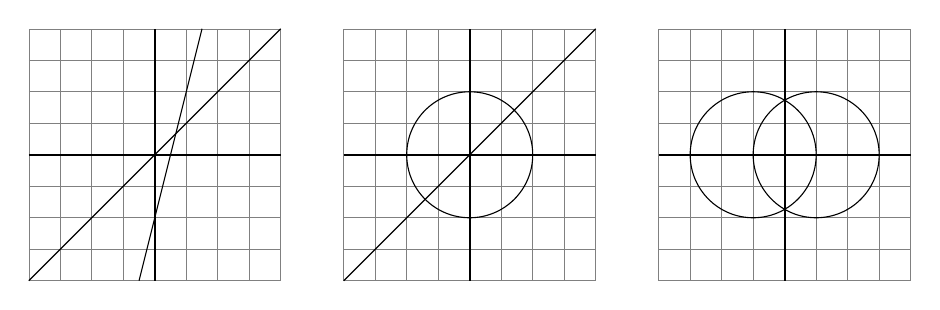
\begin{tikzpicture}[scale=.4]
\draw[step=10mm,white!50!black,very thin] (-4,-4) grid (4,4);
\draw[thick] (-4,0) -- (4,0);
\draw[thick] (0,-4) -- (0,4);
\coordinate (O) at (0,0);
\draw[name path=eq1] (-4,-4) -- (4,4);
\draw[name path=eq2] (-.5,-4) -- (1.5,4);
\path[name intersections={of=eq1 and eq2,by={P}}];
\begin{scope}[xshift=10cm]
\coordinate (O) at (0,0);
\draw[step=10mm,white!50!black,very thin] (-4,-4) grid (4,4);
\draw[thick] (-4,0) -- (4,0);
\draw[thick] (0,-4) -- (0,4);
\coordinate (A) at (2,0);
\node[draw,circle through=(A),name path=circle] at (0,0) {};
\draw[name path=eq1] (-4,-4) -- (4,4);
\path[name intersections={of=eq1 and circle,by={P,Q}}];
\end{scope}
\begin{scope}[xshift=20cm]
\coordinate (O) at (0,0);
\draw[step=10mm,white!50!black,very thin] (-4,-4) grid (4,4);
\draw[thick] (-4,0) -- (4,0);
\draw[thick] (0,-4) -- (0,4);
\coordinate (A) at (3,0);
\node[draw,circle through=(A),name path=circle1] at (1,0) {};
\coordinate (B) at (-3,0);
\node[draw,circle through=(B),name path=circle2] at (-1,0) {};
\path[name intersections={of=circle1 and circle2,by={P,Q}}];
\end{scope}
\end{tikzpicture}
\end{center}

\end{frame}

%%%%%%%%%%%%%%%%%%%%%%%%%%%%%%%%%%%%%%%%%%%%%%%%%%%%%%

\begin{frame}
\frametitle{Rationals/Square Roots Can Be Constructed}

\begin{center}
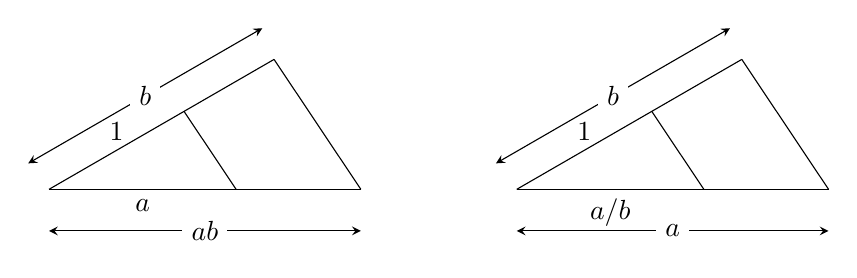
\begin{tikzpicture}[scale=.66]
\draw[name path=horz] (0,0) coordinate (o) -- (6,0);
\coordinate (a) at (6,0);
\draw (o) -- (30:5);
\coordinate (c) at (30:3);
\coordinate (b) at (30:5);
\draw (a) -- (b);
\path[name path=par] (c) -- +($(a)-(b)$);
\path[name intersections={of=par and horz,by=d}];
\draw (c) -- (d);
\draw[<->] (-.4,.5) -- node[fill=white] {$b$} +(30:5.2);
\path (o) -- node[above] {$1$} (c);
\draw[<->] (0,-.8) -- node[fill=white] {$ab$} +(6,0);
\path (o) -- node[below] {$a$} (d);
\begin{scope}[xshift=9cm]
\draw[name path=horz] (0,0) coordinate (o) -- (6,0);
\coordinate (a) at (6,0);
\draw (o) -- (30:5);
\coordinate (c) at (30:3);
\coordinate (b) at (30:5);
\draw (a) -- (b);
\path[name path=par] (c) -- +($(a)-(b)$);
\path[name intersections={of=par and horz,by=d}];
\draw (c) -- (d);
\draw[<->] (-.4,.5) -- node[fill=white] {$b$} +(30:5.2);
\path (o) -- node[above] {$1$} (c);
\draw[<->] (0,-.8) -- node[fill=white] {$a$} +(6,0);
\path (o) -- node[below] {$a/b$} (d);
\end{scope}
\end{tikzpicture}
\end{center}

\begin{center}
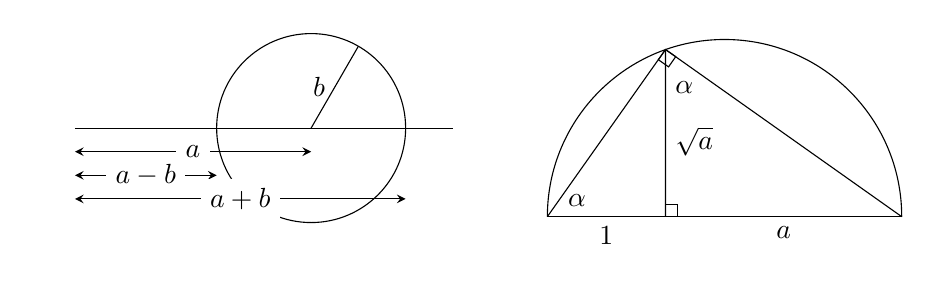
\begin{tikzpicture}[scale=.75]
\begin{scope}[scale=.8]
\clip (-1,-3) rectangle (8,2);
\coordinate (P) at (0,0);
\coordinate (Q) at (5,0);
\coordinate (T) at (3,0);
\coordinate (U) at (7,0);
\draw (P) -- (Q);
\draw (5,0) -- (8,0);
\draw (5,0) circle[radius=2cm];
\draw (5,0) -- node[left] {$b$} ++(60:2cm);
\draw[<->] (0,-.5) -- node[fill=white] {$a$} (5,-.5);
\draw[<->] (0,-1) -- node[fill=white] {$a-b$} (3,-1);
\draw[<->] (0,-1.5) -- node[fill=white] {$a+b$} (7,-1.5);
\end{scope}
\begin{scope}[xshift=8cm,yshift=-1.5cm]
\draw[name path=horz] (0,0) coordinate (a) -- (6,0);
\coordinate (b) at (6,0);
\draw[name path=circle] (b) arc(0:180:3);
\path[name path=perp] (2,0) -- +(0,3.2);
\coordinate (c) at (2,0);
\path[name intersections={of=circle and perp,by=d}];
\draw (c) -- node[right,yshift=-3pt] {$\sqrt{a}$} (d);
\path (a) -- node[below] {$1$} (c) -- node[below] {$a$} (b);
\draw (c) rectangle +(6pt,6pt);
\draw (a) -- (d) -- (b);
\draw[rotate=-125] (d) rectangle +(6pt,6pt);
\node[above right,xshift=4pt] at (a) {$\alpha$};
\node[below right,yshift=-8pt] at (d) {$\alpha$};
\end{scope}
\end{tikzpicture}
\end{center}

\end{frame}

%%%%%%%%%%%%%%%%%%%%%%%%%%%%%%%%%%%%%%%%%%%%%%%%%%%%%%

\begin{frame}
\frametitle{Constructible Regular Polygons}
\begin{center}
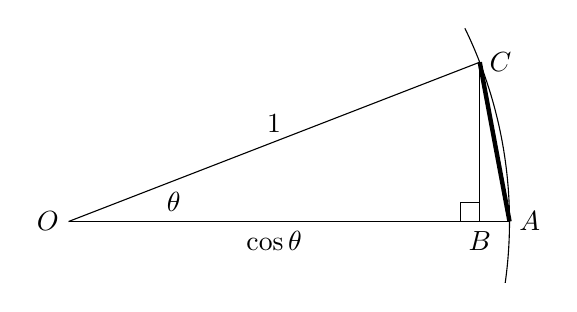
\begin{tikzpicture}[scale=1.4]
\coordinate (O) at (0,0) node[left] {$O$} node[above right,xshift=32pt] {$\theta$};
\coordinate (A) at (4,0);
\node[right] at (A) {$A$};
\draw (O) -- (A);
\draw (-8:4) arc (-8:26:4);
%\draw (A) arc(0:21.18:4);
\coordinate (C) at (21.18:4cm);
\draw (O) -- node[above] {$1$} (C);
\node[right] at (C) {$C$};
\draw (C) -- (C |- A) coordinate (B);
\node[below] at (B) {$B$};
\draw[rotate=90] (B) rectangle +(5pt,5pt);
\draw[ultra thick] (A) -- (C);
\path (O) -- node[below] {$\cos \theta$} (B); 
\end{tikzpicture}
\end{center}

\pause

Cosines of central angles of constructible polygons:
\begin{itemize}
\item Triangle: $360/3=120$ and $\cos 120=-1/2$
\item Pentagon: $360/5=72$ and $\cos 72=(\sqrt{5}-1)/4$
\item Pentadecagon: $360/15=24=(120-72)/2$
\item Bisect the central angle: $120/2^n,\; 72/2^n,\; 24/2^n$
\end{itemize}

\end{frame}

%%%%%%%%%%%%%%%%%%%%%%%%%%%%%%%%%%%%%%%%%%%%%%%%%%%%%%

\begin{frame}
\frametitle{Mathematical Prerequisites}

\pause

\begin{itemize}
\item $x^nx^m=x^{n+m}$
\pause

\medskip

\item For $n,d\neq 0$, there exist $q,r,\,0\leq r < d$ such that $n=dq+r$
\pause
\medskip
\item The roots of $x^2+bx+c$ are $(-b\pm\sqrt{b^2-4c})/2$

%\bigskip
%\item Fundamental Theorem of Algebra: $n$-th degree polynomial with complex coefficients has $n$ complex roots.
\medskip
\pause
\item $x^{17}-1$ has a root $r\neq 1$
\[
(\cos (2\pi/17) + i\,\sin  (2\pi/17))^{17} = \cos 2\pi + i\,\sin 2\pi = 1
\]
But $\pi$ is not constructible
\end{itemize}
\end{frame}

%%%%%%%%%%%%%%%%%%%%%%%%%%%%%%%%%%%%%%%%%%%%%%%%%%%%%%

\begin{frame}
\frametitle{The Roots of Unity}

\begin{itemize}
\item \textit{Definition} The roots of $x^{n}-1$ are the \emph{$n$-th roots of unity}
\medskip
\item  If $r$ is an $n$-th root of unity then $(r^{2})^n=(r^{n})^2=1^2=1$ so $r^2$ is also an $n$-th root of unity
\medskip
\item All $1, r, r^2, \ldots, r^{n-2}, r^{n-1}$ are $n$-th roots of unity
\medskip
\item Are they distinct?
\pause
\medskip
\item Not necessarily: the roots of $x^4-1$ are $1,-1,i,-i$, but:
\[
(-1)^1=-1,\;(-1)^2=1,\; (-1)^3=-1,\; (-1)^4=1
\]
\end{itemize}
\end{frame}

%%%%%%%%%%%%%%%%%%%%%%%%%%%%%%%%%%%%%%%%%%%%%%%%%%%%%%

\begin{frame}
\frametitle{Roots of Unity for $n$ Prime}

\textit{Theorem} If $n$ is a \textit{prime number} and $r$ is an $n$-the root of unity then $1,r,r^2,\ldots,r^{n-2},r^{n-1}$ are distinct.

\medskip

\textit{Proof}

If $r^{\,i}=r{\,^j}$ for $1\leq i < j \leq n-1$, then $r{\,^j}/r{\,^i}=r{\,^{j-i}}=1$.

Let $m$ be the smallest \textit{positive} integer such that $r^{m}=1$.
\[
1=r^n=r^{qm+k}=(r^m)^q\cdot r^k=1^q\cdot r^k=r^k
\]
$0\leq k<m$ and $r^k=1$. But $0<k$ contradicts the assumption on $m$, so it follows that $k=0$ and $n=mq$ is not prime.

\end{frame}

%%%%%%%%%%%%%%%%%%%%%%%%%%%%%%%%%%%%%%%%%%%%%%%%%%%%%%

\begin{frame}
\frametitle{From Roots Back to Coefficients}

If $r_1,r_2$ are roots of $x^2+bx+c$ then:
\begin{eqnarray*}
(x-r_1)(x-r_2)&=&x^2 - (r_1+r_2)x + r_1r_2=x^2+bx+c\\\\
b&=&-(r_1+r_2)\\
c&=&r_1r_2
\end{eqnarray*}
\pause
The roots of $x^{17}-1$ are $\{1,r,r^2,\cdots, r^{15}, r^{16}\}$  so:
\begin{eqnarray*}
x^{17}-1&=&(x-1)(x-r^1)(x-r^2)\cdots (x-r^{15})(x-r^{16})\\\\
\pause
0\cdot x^{16} &=& [-(1+r^1+r^2+\cdots+r^{15}+r^{16})]\cdot x^{16}\\\\
-1&=&r^1+r^2+\cdots+r^{15}+r^{16}
\end{eqnarray*}

\end{frame}

%%%%%%%%%%%%%%%%%%%%%%%%%%%%%%%%%%%%%%%%%%%%%%%%%%%%%%

\begin{frame}
\frametitle{The Heptadecagon is Constructible}
\[
\begin{array}{rrrrrrrrrrrrrrrr}
r^1\!&\! r^2\!&\! r^3\!&\! r^{4}\!&\! r^{5}\!&\! r^6\!&\! r^{7}\!&\! r^{8}\!&\! r^{9}\!&\! r^{10}\!&\! r^{11}\!&\! r^{12}\!&\! r^{13}\!&\! r^{14}\!&\! r^{15}\!&\! r^{16}
\end{array}
\]
\pause
\[
r^1, \;(r^1)^3 =r^3,\; (r^3)^3=r^9,\; (r^9)^3=r^{27}=r^{10}, \;  \;\ldots
\]
\pause
\[
\begin{array}{rrrrrrrrrrrrrrrr}
r^1\!&\! r^3\!&\! r^9\!&\! r^{10}\!&\! r^{13}\!&\! r^5\!&\! r^{15}\!&\! r^{11}\!&\! r^{16}\!&\! r^{14}\!&\! r^8\!&\! r^7\!&\! r^4\!&\! r^{12}\!&\! r^2\!&\! r^6
\end{array}
\]
\end{frame}
%%%%%%%%%%%%%%%%%%%%%%%%%%%%%%%%%%%%%%%%%%%%%%%%%%%%%%

\begin{frame}
\frametitle{The Heptadecagon is Constructible}

\[
\begin{array}{rrrrrrrrrrrrrrrr}
r^1\!&\! r^3\!&\! r^9\!&\! r^{10}\!&\! r^{13}\!&\! r^5\!&\! r^{15}\!&\! r^{11}\!&\! r^{16}\!&\! r^{14}\!&\! r^8\!&\! r^7\!&\! r^4\!&\! r^{12}\!&\! r^2\!&\! r^6
\end{array}
\]

\medskip
$a_0,a_1$ are the sums of every second root:
\begin{eqnarray*}
a_0&=&r + r^9 + r^{13} +r^{15} +r^{16} + r^8+r^4+r^2\\
a_1&=&r^3 + r^{10} + r^{5} +r^{11} +r^{14} + r^7+r^{12}+r^6\\\\
\pause
a_0+a_1&=&r^1+r^2+\cdots+r^{15}+r^{16}= -1
\end{eqnarray*}

\end{frame}

%%%%%%%%%%%%%%%%%%%%%%%%%%%%%%%%%%%%%%%%%%%%%%%%%%%%%%

\begin{frame}
\frametitle{The Heptadecagon is Constructible}
\[
\begin{array}{lcl}
a_0a_1&=&(r + r^9 + r^{13} +r^{15} +r^{16} + r^8+r^4+r^2)\;\;\times\\
&&(r^3 + r^{10} + r^{5} +r^{11} +r^{14} + r^7+r^{12}+r^6)\\\\
&=&\occ{4}{1} + \occ{11}{1} + \occ{6}{1} + \occ{12}{1} + \occ{15}{1} + \occ{8}{1} + \occ{13}{1} + \occ{7}{1} +\\
&&\occ{12}{2} + \occ{2}{1} + \occ{14}{1} + \occ{3}{1} + \occ{6}{2} + \occ{16}{1} + \occ{4}{2} + \occ{15}{2} +\\
&&\occ{16}{2} + \occ{6}{3} + \occ{1}{1} + \occ{7}{2} + \occ{10}{1} + \occ{3}{2} + \occ{8}{2} + \occ{2}{2}\;\;\: +\\
&&\occ{1}{2} + \occ{8}{3} + \occ{3}{3} + \occ{9}{1} + \occ{12}{3} + \occ{5}{1} + \occ{10}{2} + \occ{4}{3}\;\;\: +\\
&&\occ{2}{3} + \occ{9}{2} + \occ{4}{4} + \occ{10}{3} + \occ{13}{2} + \occ{6}{4} + \occ{11}{2} + \occ{5}{2} \:+\\
&&\occ{11}{3} + \occ{1}{3} + \occ{13}{3} + \occ{2}{4} + \occ{5}{3} + \occ{15}{3} + \occ{3}{4} + \occ{14}{2} \;+\\
&&\occ{7}{3} + \occ{14}{3} + \occ{9}{3} + \occ{15}{4} + \occ{1}{4} + \occ{11}{4} + \occ{16}{3} + \occ{10}{4} +\\
&&\occ{5}{4} + \occ{12}{4} + \occ{7}{4} + \occ{13}{4} + \occ{16}{4} + \occ{9}{4} + \occ{14}{4} + \occ{8}{4}\\\\
&=&-4
\end{array}
\]

\end{frame}

%%%%%%%%%%%%%%%%%%%%%%%%%%%%%%%%%%%%%%%%%%%%%%%%%%%%%%

\begin{frame}
\frametitle{The Heptadecagon is Constructible}


\begin{eqnarray*}
-(a_0+a_1)&=&1\\
a_0a_1&=&-4
\end{eqnarray*}

Let $a_0,a_1$ be roots of a quadratic equation:

\begin{eqnarray*}
y^2+y-4&=&0\\
a_0, a_1&=& \frac{-1\pm\sqrt{17}}{2}
\end{eqnarray*}

\end{frame}

%%%%%%%%%%%%%%%%%%%%%%%%%%%%%%%%%%%%%%%%%%%%%%%%%%%%%%

\begin{frame}
\frametitle{The Heptadecagon is Constructible}

\bigskip

$b_0,b_1, b_2, b_3$ are the sums of every fourth root:
\begin{eqnarray*}
b_0&=& r^1+ r^{13} + r^{16} + r^4\\
b_1&=& r^3+ r^{5} + r^{14} + r^{12}\\
b_2&=& r^9+ r^{15} + r^{8} + r^2\\
b_3&=& r^{10}+ r^{11} + r^{7} + r^6\\\\
\pause
-(b_0+b_2)&=&-a_0\\
b_0b_2&=&-1\\
-(b_1+b_3)&=&-a_1\\
b_1b_3&=&-1
\end{eqnarray*}
\end{frame}

%%%%%%%%%%%%%%%%%%%%%%%%%%%%%%%%%%%%%%%%%%%%%%%%%%%%%%

\begin{frame}
\frametitle{The Heptadecagon is Constructible}

Let $b_0,b_2$ be roots of a quadratic equation:
\begin{eqnarray*}
y^2-a_0y-1&=& 0\\
b_0&=&\frac{(-1+\sqrt{17}) + \sqrt{34-2\sqrt{17}}}{4}
\end{eqnarray*}

Let $b_1,b_3$ be roots of a quadratic equation:
\begin{eqnarray*}
y^2-a_1y-1&=& 0\\
b_1&=&\frac{(-1-\sqrt{17}) + \sqrt{34+2\sqrt{17}}}{4}
\end{eqnarray*}

\end{frame}

%%%%%%%%%%%%%%%%%%%%%%%%%%%%%%%%%%%%%%%%%%%%%%%%%%%%%%

\begin{frame}
\frametitle{The Heptadecagon is Constructible}

\bigskip

$c_0,\ldots, c_8$ are the sums of every eighth root:
\begin{eqnarray*}
c_0&=&r^1+r^{16}\\
c_4&=&r^{13}+r^4\\\\
-(c_0+c_4)&=&-b_0\\
c_0c_4&=&b_1
\end{eqnarray*}

Let $c_0,c_4$ be roots of a quadratic equation.
\[
y^2-b_0y+b_1=0
\]

\end{frame}

%%%%%%%%%%%%%%%%%%%%%%%%%%%%%%%%%%%%%%%%%%%%%%%%%%%%%%

\begin{frame}
\frametitle{The Heptadecagon is Constructible}
For $\theta=(360^\circ/17)$, $\cos\theta=(r^1+r^{16})/2= c_0/2$:

\bigskip

\begin{center}
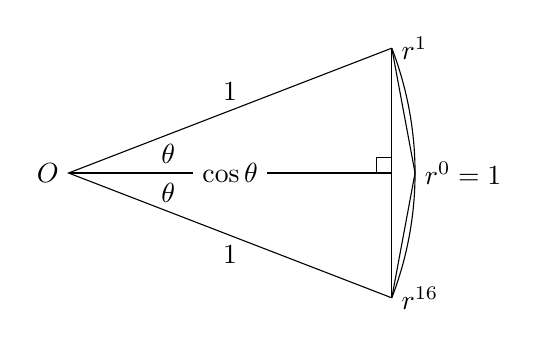
\begin{tikzpicture}[scale=1.1]
\coordinate (O) at (0,0) node[left] {$O$}
  node[above right,xshift=30pt] {$\theta$}
  node[below right,xshift=30pt] {$\theta$};
\coordinate (A) at (4,0);
\node[right] at (A) {$r^0=1$};
\coordinate (C) at (21.12:4cm);
\coordinate (D) at (-21.12:4cm);
\draw (D) arc(-21.12:21.12:4);
\draw (D) -- node[below] {$1$} (O) -- node[above] {$1$} (C);
\node[right] at (C) {$r^1$};
\node[right] at (D) {$r^{16}$};
\draw (C) -- (C |- A) coordinate (B);
\draw (D) -- (D |- A);
\draw[rotate=90] (B) rectangle +(5pt,5pt);
\draw (D) -- (A) -- (C);
\draw (O) --  node[fill=white] {$\cos \theta$} (B);
\end{tikzpicture}
\end{center}
\end{frame}

%%%%%%%%%%%%%%%%%%%%%%%%%%%%%%%%%%%%%%%%%%%%%%%%%%%%%%

\begin{frame}
\frametitle{The Heptadecagon is Constructible}
\vspace{-4ex}
\[
\begin{array}{l}
%\cos\left(\disfrac{360^\circ}{17}\right) &=& 
c_0/2=\\\\
\quad\displaystyle\frac{1}{16}+\displaystyle\frac{1}{16}\sqrt{17} + 
     \displaystyle\frac{1}{16}\sqrt{34-2\sqrt{17}}\; +\\\\
 \quad\displaystyle\frac{1}{16}\sqrt{
     68+12\sqrt{17} + 
     2(-1+\sqrt{17})\sqrt{34-2\sqrt{17}}
   -16
     \sqrt{34+2\sqrt{17}}
   }
\end{array}
\]
\bigskip

\begin{center}
\Large QED
\end{center}

\end{frame}

%%%%%%%%%%%%%%%%%%%%%%%%%%%%%%%%%%%%%%%%%%%%%%%%%%%%%%

\begin{frame}
\frametitle{Gauss-Wantzel Theorem}
\textit{Theorem} A regular polygon with $n$ sides is constructible if and only if $n$ is the product of $2^n$ and zero or more \emph{distinct} prime Fermat numbers $F_k=2^{2^k}+1$.

\bigskip
\bigskip

The known Fermat primes are:
\[
F_0=3,\quad F_1=5,\quad F_2=17,\quad F_3=257,\quad F_4=65537\,.
\]

$F_5,\ldots,F_{32}$ are \textit{not} prime.
\end{frame}

%%%%%%%%%%%%%%%%%%%%%%%%%%%%%%%%%%%%%%%%%%%%%%%%%%%%%%

\begin{frame}
\frametitle{Construction of a Heptadecagon}

The first construction was given in $1893$

\medskip

This construction is from Callagy ($1983$)

\begin{center}
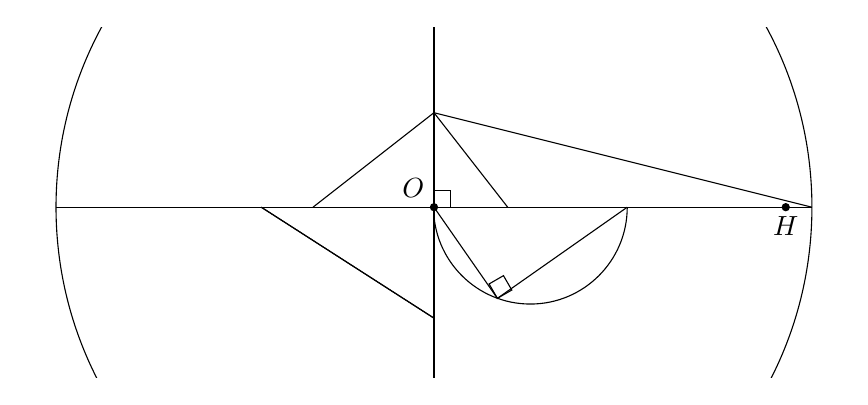
\begin{tikzpicture}[scale=1.2]
\clip (-4.3,-1.8) rectangle (4.3,1.9);
\coordinate (O) at (0,0);
\draw (O) circle (4cm);
\coordinate (P) at (4,0);
\coordinate (R) at (0,4);
\coordinate (Q) at (-4,0);
\coordinate (S) at (0,-4);
\coordinate (A) at (0,1);
\coordinate (B) at (.78,0);
\coordinate (C) at (-1.28,0);

\coordinate (D) at (.5,0);
\coordinate (E) at (2.045,0);
\coordinate (M) at (-1.8275,0);

\path[name path=circ] (M) circle (2.1725cm);
\path[name path=yaxis] (R) -- (S);
\path[name intersections={of=circ and yaxis,by={F1,F}}];
\draw (M) -- (F);

\draw[name path=OEarc] (E) arc(0:-180:1.025cm);
\path[name path=OFcircle] (O)
  let
    \p1 = ($(O)-(F)$)
  in
    circle({veclen(\x1,\y1)});
\path[name intersections={of=OEarc and OFcircle, by={G}}];
\draw (O) -- (G) -- (E);
\path (O) -- (F);

\path[name path=EGcircle] (E) 
  let
  \p1 = ($(E)-(G)$)
  in
    circle({veclen(\x1,\y1)});
\draw[name path=PQ] (P) -- (Q);
\path[name intersections={of=PQ and EGcircle, by={H,H1}}];
\path (E) -- (H);

\draw (R) -- (S);
\draw (A) -- (P);
\draw (C) -- (A) -- (B);
\draw (M) -- (F);
\vertex{H};
\node[above left] at (O) {$O$};
\node[below] at (H) {$H$};
\vertex{O};
\draw (O) rectangle +(+5pt,+5pt);
\draw[rotate=30] (G) rectangle +(+5pt,+5pt);
\path (Q) -- (M);
\end{tikzpicture}

\bigskip

$\overline{OH}=\cos (360^\circ/17)$
\end{center}

\end{frame}

%%%%%%%%%%%%%%%%%%%%%%%%%%%%%%%%%%%%%%%%%%%%%%%%%%%%%%

\begin{frame}
\frametitle{A Farewell to Algebra\\
(Apologies to Ernest Hemingway)}
\begin{Large}
Dear Algebra,

\bigskip

Please stop asking us to find your \textbf{\Large X}.

\bigskip

She's never coming back and don't ask \textbf{\Large Y}.
\end{Large}
\end{frame}

\begin{frame}

\begin{center}
\vspace*{-5ex}
\includegraphics[height=7cm]{mosteller-cover}
\end{center}

\medskip

\small\url{https://github.com/motib/probability-mosteller}

\end{frame}


\end{document}
